\documentclass{standalone}

\usepackage{tikz}
\usepackage{amssymb}
\usetikzlibrary{calc, positioning, shapes.geometric}

\begin{document}
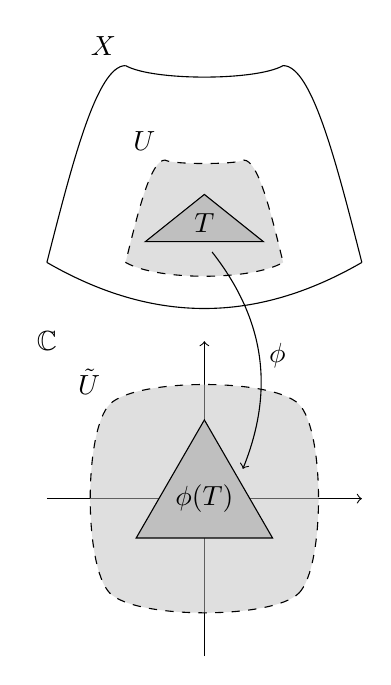
\begin{tikzpicture}
	\coordinate (a) at (-2,-2);
	\coordinate (b) at (2,-2);
	\coordinate[label=above left:{$ X $}] (c) at (-1,0.5);
	\coordinate (d) at (1,0.5);
	\draw[bend right] (a) to (b);
	\draw[bend right, looseness=0.5] (c) to (d);
	\draw (b) sin (d);
	\draw (a) sin (c);

	\coordinate (t) at (0,-1.5);
	\coordinate (Ua) at ($ (t) + (-1,-0.5) $);
	\coordinate (Ub) at ($ (t) + (1, -0.5) $);
	\coordinate[label=above left:{$ U $}] (Uc) at ($ (t) + (-0.5, 0.8) $);
	\coordinate (Ud) at ($ (t) + (0.5, 0.8) $);

	\filldraw[dashed, fill=gray!50, fill opacity=0.5] (Ua) to[bend right, looseness=0.6] (Ub) sin
	(Ud) to[bend left, looseness=0.3] (Uc) cos cycle;

	\node[isosceles triangle, isosceles triangle stretches, shape border
		rotate=90, minimum width=1.5cm, minimum height=0.6cm, draw, label={center:$
					T $}, fill=gray!50] (T) at (t) {};

	\begin{scope}[yshift=-5cm]
		\draw[->] (-2,0) to (2,0);
		\draw[->] (0,-2) to (0,2);
		\node at (-2,2){$ \mathbb{C} $};

		\draw[dashed, fill=gray!50, fill opacity=0.5] plot[smooth cycle] coordinates {(-1.2,-1.2)
				(1.2,-1.2) (1.2,1.2) (-1.2,1.2)};
		\node[above left] at (-1.2,1.2) {$ \tilde{U} $};
		\node[regular polygon, regular polygon sides=3, minimum size=2cm,
			label={center:$ \phi(T) $}, draw, fill=gray!50] (fT) at (0,0)
		{};
	\end{scope}

	\node (top) at (T.south){};
	\node (bottom) at (fT.side 3){};
	\draw[->, bend left] (top) to node[right]{$ \phi $} (bottom);

\end{tikzpicture}
\end{document}
